\chapter{\MakeUppercase{System Design}}
\justifying

\section{System Architecture}\label{sec:sysarch}

The AI Health Screening Assistant follows a client-server architecture comprising three distinct layers: a Streamlit-based frontend, a FastAPI-based backend orchestration engine, and three PyTorch inference modules. Figure 4.1 presents the high-level system architecture.

\begin{figure}[h!]
	\centering
	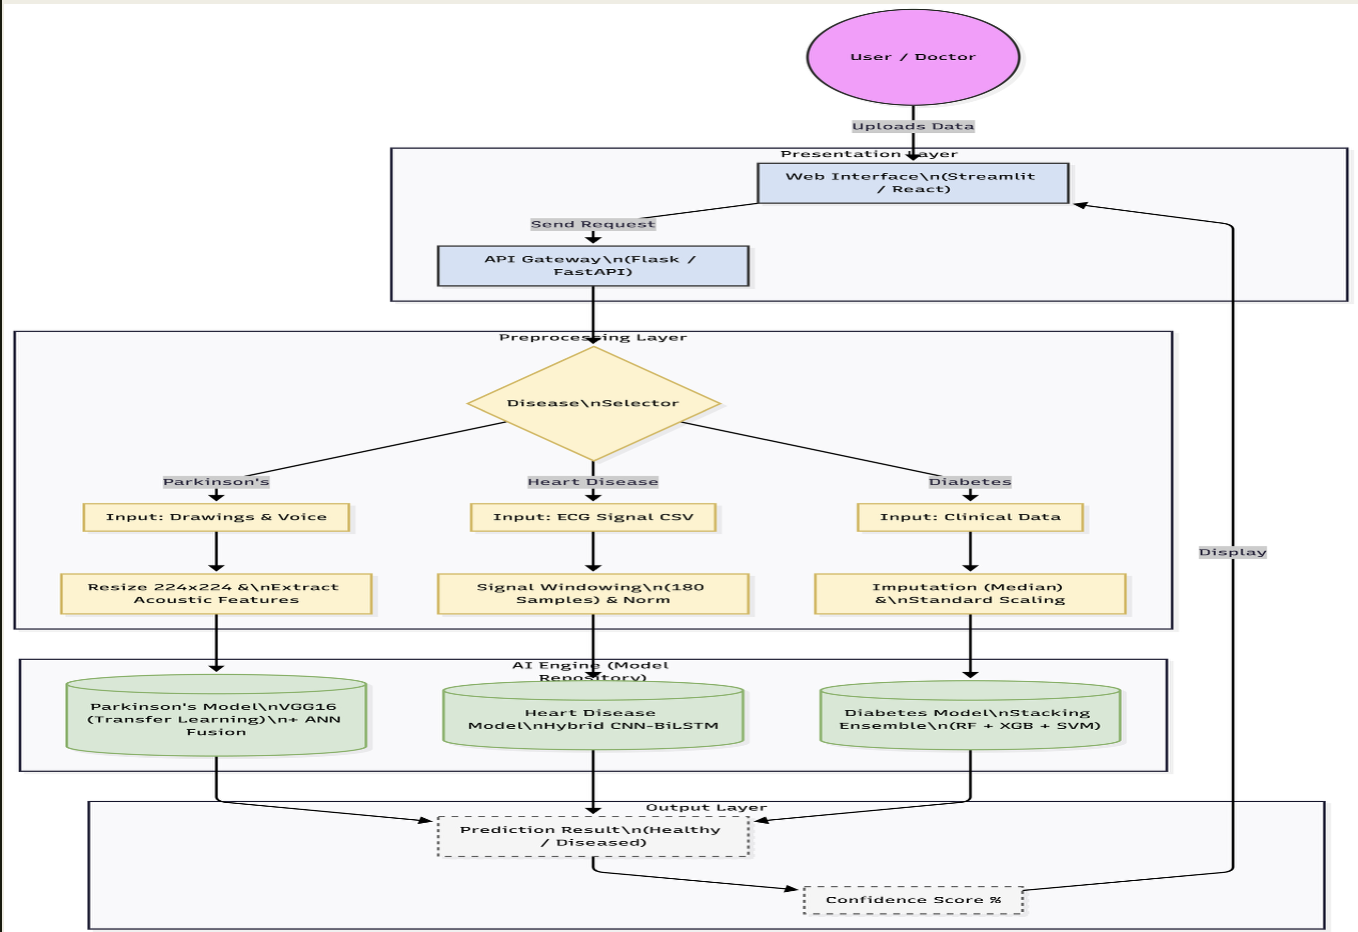
\includegraphics[width=0.85\linewidth]{images/system_diagram.png}
	\caption[High-Level System Architecture]{High-Level System Architecture of the AI Health Screening Assistant}
	\label{fig:sysarch}
\end{figure}

The system is designed around a novel \textbf{double-pass \ac{llm}} pattern. In the first pass, the Gemini \ac{llm} conducts a structured medical intake interview, collecting patient data conversationally and terminating with a structured \texttt{<MODEL\_INPUT>} XML block. The backend intercepts this block, parses it, and routes the data to the appropriate inference modules. After all three models have produced risk scores, the backend constructs a \texttt{<MODEL\_OUTPUT>} block and initiates a second pass to Gemini, which interprets the quantitative results and generates an empathetic patient-facing explanation.

This architecture ensures that \textbf{the \ac{llm} never fabricates risk probabilities} — all numerical predictions originate exclusively from the PyTorch models.

\subsection{Frontend (Streamlit)}

The Streamlit frontend (\texttt{ui/streamlit\_app.py}) provides:
The Streamlit frontend, implemented in \texttt{ui/streamlit\_app.py}, securely establishes the primary user experience through several integrated UI components. Central to the application is a deeply integrated chat interface functioning via \texttt{st.chat\_message} and \texttt{st.chat\_input} bindings, enabling fluid two-way \ac{llm} interaction. This is structurally supported by a dedicated sidebar containing specialised file upload widgets explicitly configured to ingest \ac{ecg} data in CSV format and motor analysis recordings in WAV or MP3 formats. Throughout the interaction, users are visually informed of background processing via a real-time display capturing the current screening status (pending, in progress, or completed). Upon concluding the pipeline inference, the interface natively renders interactive risk badges dynamically showcasing isolated cardiac, metabolic, and motor risk levels utilising intuitive clinical colour-coding schemes. Finally, the application securely tops the dashboard with a universal triage level indicator decisively characterising the patient's immediate medical urgency as strictly routine, requiring a recommended check, or mandating a priority review.

\subsection{Backend (FastAPI)}

The FastAPI backend (\texttt{app.py}) exports four endpoints and pre-loads all three \ac{dl} models at startup via the \texttt{@app.on\_event("startup")} handler, ensuring zero cold-start inference latency for subsequent requests.

The backend's internal \textbf{orchestration flow} executing within the FastAPI \texttt{/chat} endpoint follows a deeply systematic cycle. To initiate the sequence, the script systematically appends internal upload status flags onto the most recent user message strings, a technique designed explicitly to prevent the inference-stage \ac{llm} from redundantly requesting files that have already been securely ingested. Once contextualised, the engine sequentially fires a call to the Gemini \ac{llm} handler established within \texttt{chat/groq\_client.py}. It concurrently scans the resulting textual stream for the critical \texttt{<MODEL\_INPUT>} structural tags operating via regex extraction. If this structural block is positively detected, the sequence halts the chat flow, mathematically parses the extracted XML nodes, triggers parallel execution across all three loaded \ac{dl} inference modules, and subsequently constructs a rigid \texttt{<MODEL\_OUTPUT>} block containing the neural probabilities. Possessing this empirical data, the backend immediately forces a critical second Gemini \ac{api} call armed securely with the new PyTorch inference dictionary precisely to generate the highly empathetic patient-facing explanation. Upon successfully compiling the \ac{llm} textual conclusions with the mathematical model probabilities, the server securely returns the final packaged explanation strictly to the Streamlit frontend.

\subsection{Inference Modules}

Each inference module (\texttt{inference/heart.py}, \texttt{inference/diabetes.py}, \texttt{inference/parkinson.py}) is self-contained, implementing both the model architecture class and the \texttt{predict()} function. Models are cached as module-level singletons and loaded lazily on first call (or at startup). All modules use PyTorch's \texttt{torch.no\_grad()} context for inference to suppress gradient computation.

\subsection{LLM Integration (Gemini)}

The \texttt{chat/groq\_client.py} module implements the Gemini client with:
Operating internally, the \texttt{chat/groq\_client.py} module meticulously implements the Gemini \ac{api} client bounded by rigid operational safety logic. It enforces a strict foundational medical system prompt entirely encoding the precise data collection protocols, the imperative \ac{ai} safety guardrails, alongside exhaustive XML output format specifications guaranteeing downstream data sanitation. To safeguard against inevitable cloud rate limits, the module executes a native three-stage architectural fallback chain automatically cascading requests from the highly performant gemini-1.5-flash endpoint down toward the gemini-1.5-pro tier, before optionally bottoming out strictly at gemini-2.0-flash. Should insurmountable \ac{api} downtimes cascade through the entire Google ecosystem, the client intrinsically handles a secondary global HuggingFace inference fallback natively leveraging \texttt{Qwen/Qwen2.5-72B-Instruct} perfectly ensuring absolute, uninterrupted clinical service orchestration.

\section{Detailed Design}

\subsection{ECG Signal Processing Pipeline}\label{sec:ecg_pipeline}

The ECG preprocessing pipeline, implemented in \texttt{inference/heart.py}, consists of four stages:

The detailed \ac{ecg} preprocessing pipeline inherently implemented within \texttt{inference/heart.py} functionally executes across four sequential stages. The process begins with \textbf{Bandpass Filtering}, employing a 4th-order Butterworth bandpass filter configured precisely to a 0.5--40 Hz passband via \texttt{scipy.signal.butter} alongside zero-phase \texttt{filtfilt} application. This critical stage reliably eliminates low-frequency baseline wander (typically oscillating below 0.5 Hz) while effectively truncating high-frequency electromyographic noise and extraneous muscle artefacts resonating above 40 Hz. The sanitised signal then proceeds into \textbf{R-Peak Detection}, wherein \texttt{scipy.signal.find\_peaks} is rigidly applied using a constrained minimum inter-peak distance of 180 temporal samples (equating identically to 0.5 seconds natively at 360 Hz) alongside an adaptive dynamic height threshold established structurally at $\mu + 0.5\sigma$. Should this primary algorithmic sweep fail to detect peaks, the constraint parameters are dynamically relaxed; if the array remains stubbornly empty, the signal midpoint computationally assumes the absolute fallback position. Having isolated the ventricular contractions, the pipeline initiates \textbf{Beat Segmentation}. For each confirmed R-peak, an exact fixed temporal window is algorithmically extracted: capturing 108 samples immediately pre-R (0.3 s) combined identically with 144 samples tracking post-R (0.4 s), ultimately yielding a strictly uniform 252-sample waveform beat window. Anomalous beats artificially truncated by the signal boundaries lacking sufficient pre- or post-samples are immediately discarded from the mathematical stack. Completing the computational lifecycle is the \textbf{Batch Inference} phase. All successfully extracted sequential beats are mathematically stacked vertically into a multi-dimensional PyTorch batch tensor possessing the explicit shape (B, 1, 252) and passed parallelly through the ECGNet deep architecture. The resulting per-beat discrete softmax probability vectors are then mathematically averaged uniformly across all identified beats within the trace, definitively defining the final sequence abnormality probability strictly as $1 - P(\text{Normal})$.

\begin{algorithm}
\caption{ECG Beat Segmentation and Batch Inference}\label{alg:ecg}
\begin{algorithmic}
    \Require Filtered ECG signal $s$, sampling rate $f_s = 360$ Hz, model $\mathcal{M}$
    \Ensure Abnormality probability $p_{\text{abn}} \in [0, 1]$
    \State $\text{peaks} \gets \textsc{FindPeaks}(s,\ \text{min\_dist}=180,\ \text{height}=\mu_s + 0.5\sigma_s)$
    \State $\text{beats} \gets [\ ]$
    \For{each peak $r$ in $\text{peaks}$}
        \If{$r - 108 \geq 0$ \textbf{and} $r + 144 \leq |s|$}
            \State $\text{beats.append}(s[r-108 : r+144])$
        \EndIf
    \EndFor
    \State $B \gets \textsc{Stack}(\text{beats})$  \Comment{shape: $(N, 1, 252)$}
    \State $\text{logits} \gets \mathcal{M}(B)$
    \State $\bar{p} \gets \textsc{Mean}(\textsc{Softmax}(\text{logits}),\ \text{axis}=0)$
    \State \Return $p_{\text{abn}} = 1 - \bar{p}[\text{N\_class}]$
\end{algorithmic}
\end{algorithm}

\subsection{Voice Feature Extraction Pipeline}

The voice analysis pipeline, implemented in \texttt{inference/parkinson.py}, extracts all 22 UCI-compatible biomarkers from a WAV file using librosa:

\begin{table}[h!]
\centering
\caption{Voice Feature Extraction Methods}
\renewcommand{\arraystretch}{1.3}
\begin{tabular}{|l|l|>{\raggedright\arraybackslash}p{6.5cm}|}
\hline
\textbf{Feature Group} & \textbf{Method} & \textbf{Features} \\
\hline
Fundamental Frequency & pYIN (librosa.pyin) & Fo, Fhi, Flo \\
Frequency Perturbation & Period-to-period analysis & Jitter(\%), Jitter(Abs), RAP, PPQ, DDP \\
Amplitude Perturbation & RMS amplitude analysis & Shimmer, Shimmer(dB), APQ3, APQ5, APQ, DDA \\
Noise Ratios & Harmonic separation & NHR, HNR \\
Nonlinear Dynamics & Custom NumPy & RPDE, DFA, D2 \\
Pitch Entropy & F0 distribution & spread1, spread2, PPE \\
\hline
\end{tabular}
\end{table}

\begin{algorithm}
\caption{Voice Feature Extraction Pipeline (ParkinsonNet)}\label{alg:voice}
\begin{algorithmic}
    \Require WAV audio file path, ParkinsonNet model $\mathcal{P}$
    \Ensure Motor risk probability $p_{\text{motor}} \in [0, 1]$
    \State Load audio at 22{,}050 Hz using librosa; resample if needed
    \State $f_0,\ \text{voiced} \gets \textsc{pYIN}(\text{audio})$ \Comment{probabilistic YIN pitch estimator}
    \State $f_0^{\text{voiced}} \gets f_0[\text{voiced}]$ \Comment{keep only voiced frames}
    \State $\text{Fo} \gets \text{mean}(f_0^{\text{voiced}})$; $\text{Fhi} \gets \max(f_0^{\text{voiced}})$; $\text{Flo} \gets \min(f_0^{\text{voiced}})$
    \State Compute period-to-period differences $\Delta T_k = T_{k+1} - T_k$ on voiced periods
    \State $\text{Jitter}(\%) \gets \frac{\text{mean}(|\Delta T_k|)}{\text{mean}(T_k)} \times 100$; compute RAP, PPQ, DDP similarly
    \State Compute RMS amplitude frames; derive Shimmer, APQ3, APQ5, APQ, DDA
    \State $\text{HNR} \gets \textsc{HarmonicToNoiseRatio}(\text{audio})$; $\text{NHR} \gets 1/\text{HNR}$
    \State Compute RPDE, DFA, D2 via NumPy nonlinear dynamics implementations
    \State Compute spread1, spread2, PPE from $f_0$ entropy
    \State $\mathbf{v} \gets [\text{Fo},\ \text{Fhi},\ \text{Flo},\ \text{Jitter},\ \ldots,\ \text{PPE}]^\top \in \mathbb{R}^{22}$
    \State $\mathbf{v}^{\prime} \gets (\mathbf{v} - \boldsymbol{\mu}) / (\boldsymbol{\sigma} + \varepsilon)$ \Comment{StandardScaler normalisation}
    \State \Return $p_{\text{motor}} = \sigma(\mathcal{P}(\mathbf{v}^{\prime}))$
\end{algorithmic}
\end{algorithm}

\subsection{Diabetes Feature Normalisation}

Diabetes features collected via the \ac{llm} are normalised using pre-computed dataset statistics (stored as NumPy arrays in \texttt{inference/diabetes.py}):

\begin{equation}
	x^{\prime}_i = \frac{x_i - \mu_i}{\sigma_i + \epsilon}
\end{equation}

where $\mu_i$ and $\sigma_i$ are the training-set mean and standard deviation of feature $i$, and $\epsilon = 10^{-8}$ prevents division by zero.

\begin{algorithm}
\caption{DiabetesNet Inference Pipeline}\label{alg:diabetes}
\begin{algorithmic}
    \Require Feature dictionary $D$ with 8 biomarker values from LLM, DiabetesNet model $\mathcal{D}$
    \Ensure Metabolic risk probability $p_{\text{meta}} \in [0, 1]$
    \State $\mathbf{x} \gets [D[\text{pregnancies}],\ D[\text{glucose}],\ D[\text{bp}],\ D[\text{skin}],\ D[\text{insulin}],\ D[\text{bmi}],\ D[\text{dpf}],\ D[\text{age}]]^\top$
    \For{each $x_i$ in $\mathbf{x}$}
        \If{$x_i$ is missing or invalid} \State $x_i \gets 0.0$ \Comment{safe default}
        \EndIf
    \EndFor
    \State $x^{\prime}_i \gets (x_i - \mu_i) / (\sigma_i + 10^{-8})$ for $i = 1, \ldots, 8$
    \State $\text{logit} \gets \mathcal{D}(\mathbf{x}^{\prime})$ \Comment{forward pass under \texttt{torch.no\_grad()}}
    \State $p_{\text{meta}} \gets \sigma(\text{logit})$
    \If{$p_{\text{meta}} < 0.35$} \Return \texttt{low}
    \ElsIf{$p_{\text{meta}} < 0.70$} \Return \texttt{borderline}
    \Else{} \Return \texttt{elevated}
    \EndIf
\end{algorithmic}
\end{algorithm}

\subsection{Triage Logic}

Risk levels from the three models are combined using a rule-based triage classifier:

Discrete risk assessment outputs extrapolated structurally from the three parallel foundational deep learning models are definitively combined using an immutable rule-based triage classifier matrix. Statistically, if any single categorical classification generated across the inference layer identifies as either explicitly \textit{high} concerning cardiac anomalies, strictly \textit{elevated} regarding metabolic risk, or definitively \textit{high} isolating motor dysfunction, the pipeline immediately triggers a universal \texttt{priority\_review} state flag. Conversely, if no upper-echelon thresholds are shattered yet the algorithmic evaluations conclude that two or distinctly independent risk factors intrinsically sit simultaneously within the \textit{moderate}, \textit{borderline}, or \textit{mild} spectrums, the server systematically initiates a \texttt{recommended\_check} alert. Operating fundamentally as the baseline catch-all constraint natively, if the evaluated patient metrics fail completely to trigger either the single-variable acute flag or the multi-variable secondary heuristic cascade, the platform safely concludes the operational lifecycle universally reporting a \texttt{routine} clearance classification.

\begin{figure}[h!]
\centering
\begin{tikzpicture}[
  node distance=1.4cm,
  decision/.style={diamond, draw, fill=orange!20, text width=3.6cm, text centered,
                   inner sep=2pt, font=\small, aspect=2},
  result/.style={rectangle, draw, rounded corners=3pt, minimum width=3.4cm,
                 minimum height=0.65cm, text centered, font=\small},
  start/.style={rectangle, draw, rounded corners=3pt, fill=blue!12,
                minimum width=5.0cm, minimum height=0.65cm, text centered, font=\small},
  arrow/.style={->, >=stealth, thick}
]
\node[start] (in)   {3 Risk Scores: Cardiac, Metabolic, Motor};
\node[decision, below=1.2cm of in] (d1) {Any risk\\is \textbf{High} /\\\textbf{Elevated}?};
\node[result, right=2.6cm of d1, fill=red!20]    (p)  {\textbf{priority\_review}};
\node[decision, below=1.4cm of d1] (d2) {$\geq$2 risks are\\Moderate /\\Borderline / Mild?};
\node[result, right=2.6cm of d2, fill=yellow!35] (r)  {\textbf{recommended\_check}};
\node[result, below=1.2cm of d2,  fill=green!20] (ro) {\textbf{routine}};
\draw[arrow] (in)  -- (d1);
\draw[arrow] (d1)  -- node[above, font=\small]{Yes} (p);
\draw[arrow] (d1)  -- node[right, font=\small]{No}  (d2);
\draw[arrow] (d2)  -- node[above, font=\small]{Yes} (r);
\draw[arrow] (d2)  -- node[right, font=\small]{No}  (ro);
\end{tikzpicture}
\caption[Rule-Based Triage Decision Logic]{Rule-Based Triage Decision Logic}
\label{fig:triage}
\end{figure}

\begin{algorithm}
\caption{Rule-Based Triage Classification}\label{alg:triage}
\begin{algorithmic}
    \Require Cardiac risk $r_c$, Metabolic risk $r_m$, Motor risk $r_o$ (string labels)
    \Ensure Triage level $\in$ \{\texttt{routine}, \texttt{recommended\_check}, \texttt{priority\_review}\}
    \State $H \gets$ \{\texttt{high}, \texttt{elevated}\} \Comment{high-severity set}
    \State $M \gets$ \{\texttt{moderate}, \texttt{borderline}, \texttt{mild}\} \Comment{moderate-severity set}
    \If{$r_c \in H$ \textbf{or} $r_m \in H$ \textbf{or} $r_o \in H$}
        \State \Return \texttt{priority\_review}
    \EndIf
    \State $\text{count} \gets |\{r \in \{r_c, r_m, r_o\} : r \in M\}|$
    \If{$\text{count} \geq 2$}
        \State \Return \texttt{recommended\_check}
    \EndIf
    \State \Return \texttt{routine}
\end{algorithmic}
\end{algorithm}

\subsection{Data Flow Diagram}

Figure~\ref{fig:llmpipeline} illustrates the complete data flow from user input to screening report. The double-pass \ac{llm} architecture is the central design novelty: the \ac{llm} never generates risk numbers, only interprets them.

\begin{figure}[h!]
	\centering
	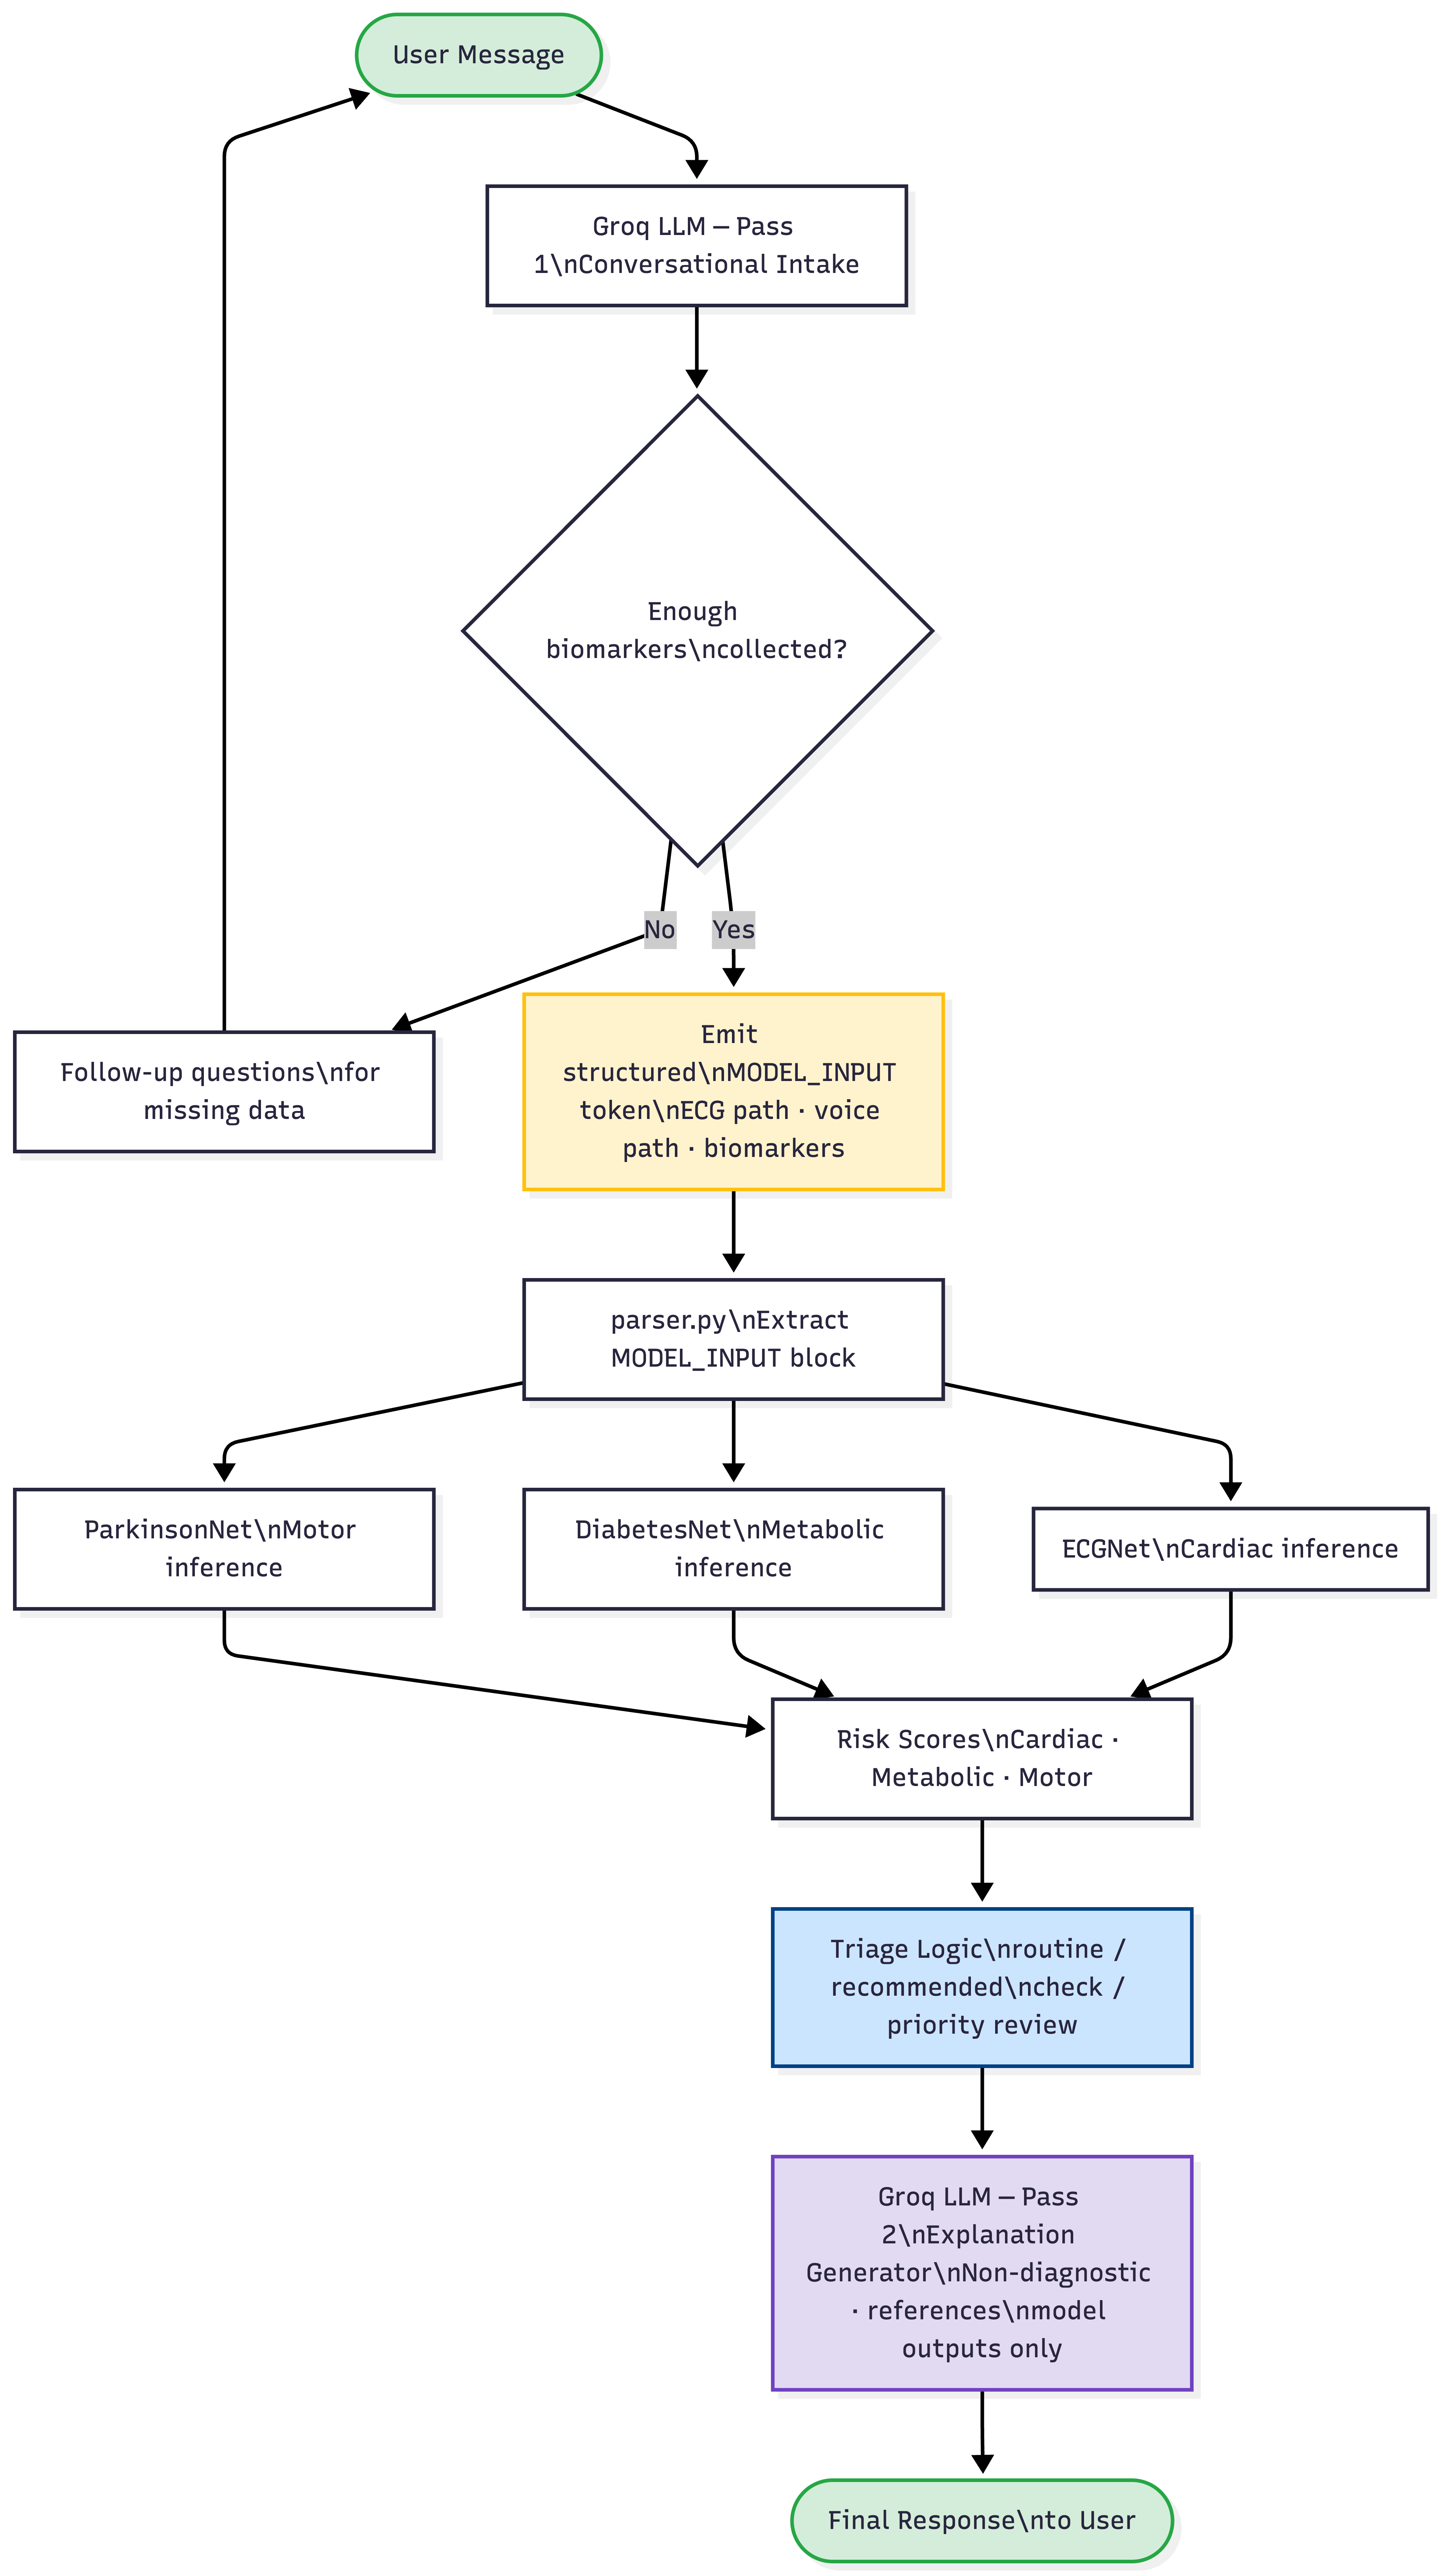
\includegraphics[width=0.95\linewidth]{images/llm_pipeline.png}
	\caption[Double-Pass LLM Pipeline]{Double-Pass LLM Pipeline --- Complete Data Flow from User Input to Screening Report}
	\label{fig:llmpipeline}
\end{figure}

